Climate change, among other environmental challenges, is (mostly) due to the concentration of anthropogenic \acrfull{GHG} in the environment \cite{IPCC_CO2_budget}. Therefore, the \gls{GHG} emissions from human activities must be mitigated to prevent further environmental damages. Among these emissions, globally, about 75\% are directly related to the whole-energy system \cite{ourworldindata_CO2_world}. The \gls{GHG} emissions, usually expressed in kt$_{\ce{CO2},\text{eq}}$, could be developed as an adapted, \ie less economy-oriented, version of the original Kaya identity \cite{kaya1997environment}:

\begin{equation}
\label{eq:equality_GHG}
\mathrm{GHG} =  \frac{\mathrm{GHG}}{\text{Primary energy}} \times \frac{\text{Primary energy}}{\mathrm{EUD}}\times \frac{\mathrm{EUD}}{\text{Population}} \times \text{Population,}\\
 \end{equation}

\noindent
where the first term represents the \gls{GWP} of the primary energy mix, the second is the inverse of the efficiency and the third stands as the energy intensity per capita. Such an identity, mathematically-correct though, is criticized for the arbitrary choice of variables, the non-independence of them usually leading to the rebound effect and its encompassing approach that does not translate properly the heterogeneity of the situation \cite{IPCC2000}. However, Eq. \ref{eq:equality_GHG} has the merit to highlight three levers of action that should be activated to reduce the \gls{GHG} emissions and, consequently, favour the transition, considering that the population will continue to grow \cite{dodson2020population,scovronick2017impact}. These three levers of actions are: renewables, efficiency and sufficiency aiming at reducing the first, the second and the third terms on the right-hand side of Eq. \ref{eq:equality_GHG}, respectively. The latter, explicitly mentioned by the IPCC for the first time in 2022 \cite{IPCC2022}, is defined by \citet{lage2023citizens} as ``a strategy for reducing, in absolute terms, the consumption and production of end-use products and services through changes in social practices in order to comply with environmental sustainability while ensuring an adequate social foundation for all people''. Altough this finds a growing interest in the scientific community \cite{o2018good}, it requires, maybe more than the two other levers, interdisciplinarity \cite{schmidt2015interdisciplinary}, \ie the combination of multiple academic disciplines like sociology, psychology or politics, that are out of the scope of my expertise, and, consequently, this thesis. However, the work developed in the present manuscript aims at providing support to such interdisciplinary projects to assess sufficiency policies. More within the grasp of the engineering world, this thesis rather focuses on the first two terms of Eq. \ref{eq:equality_GHG}, \ie renewables and efficiency. This aligns with the current European policies binding the Member States of the European Union. For instance, the Renewable Energy Directive (RED) III, published in October 2023 \cite{REDIII}, highlights that ``the Union’s climate neutrality objective (by 2050) requires a just energy transition which leaves no territory or citizen behind\footnote{This directly relates to sufficiency as it encompasses social justice in parallel with a minimization of the energy use.}, an increase in energy efficiency and significantly higher shares of energy from renewable sources in an integrated energy system'' (\ie 42.5\% of the Union's gross final consumption of energy by 2030). 

\section*{Context and motivations}

To ensure the energy supply of an assumably more and more demanding society in a context of environmental crisis, major transformations are needed (see Figure \ref{fig:intro:IEA_WEO_2019}). Besides behavioral changes, an overall reshape of the energy system is necessary in terms of primary energy sources and technologies used to convert more efficiently these resources into the \gls{EUD} (\ie the energy service required by the the final consumer) \cite{iea2020world,luderer2018residual}. The former corresponds to a whole ``fuel switch'' (see Figure \ref{fig:intro:IEA_WEO_2019}) where energy carriers called, in the literature, ``\emph{biofuels}'', ``\emph{electrofuels}'', ``\emph{synthetic fuels}'', ``\emph{renewable fuels}'' or even ``\emph{sustainable fuels}'', will more and more play a crucial role. Even if the share of electricity increases in the energy system through the electrification of the end-use demand, gaseous and liquid fuels will keep on being big players during (and after) the energy transition \cite{Ahlgren2012}. To avoid the confusion between these fuels and thereby reduce misunderstanding in political or academic discussions, we have developed a comprehensive and harmonised taxonomy (see Appendix \ref{app:Taxonomy}). In the rest of this thesis, the electro - and bio - fuels are considered as renewable and with no \gls{GWP}.  

\begin{figure}[ht!]
\centering
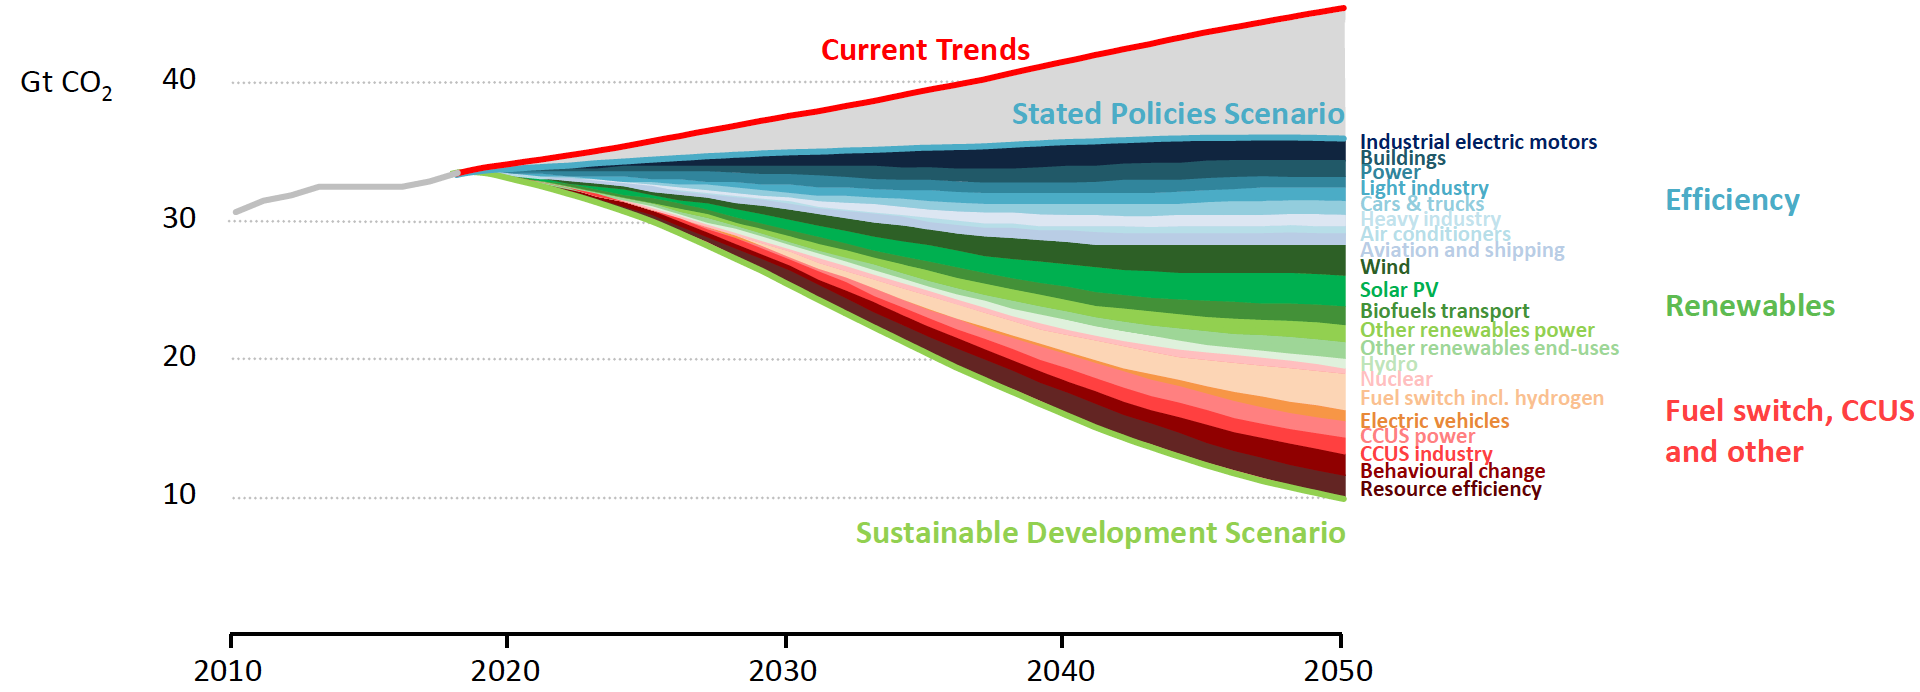
\includegraphics[width=\textwidth]{IEA_WEO_2019.png}
\caption{Energy-related CO2 emissions and reductions by sources in the Sustainable Development Scenario \cite{iea2020world}.}
\label{fig:intro:IEA_WEO_2019}
\end{figure}

In the general perspective to decrease the \gls{GWP} of the primary energy mix, \gls{VRES}, like wind and solar, have already emerged as the keystone to defossilise\footnote{Hydrocarbons, currently produced from fossil resources, will still be composed of carbon in a renewable world. This is why this thesis rather uses ``defossilisation'' rather than ``decarbonisation'' as carbon will still play a key role in a carbon-neutral energy transition \cite{mertens2020carbon}.} the energy system. However, their intermittency and space disparity could hold back their vaster integration in the future. To address this issue, due to some limitations (\eg range, power, costs) of electricity-focused solutions like \gls{DC} lines, the transport and long-term storage of the renewable electricity produced in excess should be optimised. This challenge can be tackled by \textit{electrofuels} \cite{rozzi2020}. These fuels represent energy carriers where electricity has the major share in the energy balance of the fuel. In practice, this electricity is mainly converted into hydrogen (\ie electrolysis) and then potentially upgraded into more complex fuels (\eg methane, methanol or ammonia). They offer three main advantages: infrastructure compatibility, storage and capacity to link sectors (\ie from electricity to mobility, heat, or industry). Development on electrofuels aims at getting them more and more compatible with existing and mature technologies \cite{Ahlgren2012}. An example is carbon-free ammonia-hydrogen blends burned in spark ignition engines \cite{lhuillier2020experimental} or \gls{CHP} applications \cite{pochet202022}. Moreover, some applications (\eg marine, aviation and heavy-duty transport) will be hard to electrify and keep on requiring high-density energy carriers \cite{horvath2018techno, brynolf2018}.  Then, about storage, gas networks present much more storage potential than electrical network (\eg 50 times more in Germany and 300 times more in France) \cite{Rosa2017}. Where batteries exhibit limited storage capacity (up to 10\,MWh) as well as self-discharge losses, electrofuels are an economical solution for high capacity (from 100 GWh) and long-term (\ie from months to years) storage of energy \cite{child2018role, dias2020energy} (see Figure \ref{fig:intro:Storage_electrofuels}). In their analysis of the German transport sector in 2050, \citet{millinger2021electrofuels} highlighted that producing electrofuels can represent a better usage of the ambient \ce{CO2} than \gls{CCS} to supply hydrocarbon fuels while limiting the curtailment of \gls{VRES}.  Finally, with a growing share of \gls{VRES}, sector coupling is essential to absorb the surplus of electricity from these intermittent production means \cite{robinius2017linking} and integrate them more cost-effectively \cite{brown2018response, limpensECOS2021}. Besides direct electrification of other sectors (\eg electrical heat pumps, \gls{BEV}), \citet{brown2018synergies} showed that converting power to hydrogen and methane was advantageous at high shares of renewables, in their optimisation of the European whole-energy system. Electrofuels have the ability to couple energy and non-energy sectors \cite{Stancin2020}. For instance, electricity produced in excess from \gls{VRES} can be converted into ammonia through the Haber-Bosch process and subsequently transformed into fertiliser - coupling the power and industry sectors \cite{verleysen2020can}. 

\begin{figure}[htbp!]
\centering
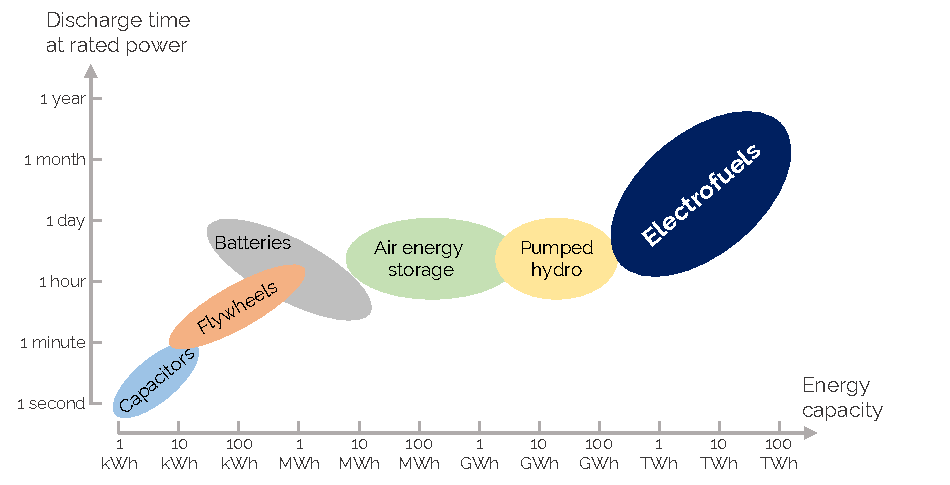
\includegraphics[width=0.9\textwidth]{Storage_electrofuels.pdf}
\caption{Energy carriers and technologies to store electricity. Electrofuels provide a solution for high capacity and long-term storage of energy. Graph adapted from \cite{ISPT2017}.}
\label{fig:intro:Storage_electrofuels}
\end{figure}

To harvest the maximum potential of synthetic energy carriers in a sustainable transition and maximise the overall system efficiency \cite{mathiesen2015}, it is necessary to study the integration of these fuels within a multi-sector and whole-energy system \cite{contino2020whole}. To reach this goal, an energy system optimisation model (ESOM) can optimise the design and the operation of the system to minimise, for instance, its costs or its emissions \cite{zeng2011review}. 

In this research field of energy system planning and scenario analysis, \citet{yue2018review} highlighted that most ESOMs use a deterministic approach (\ie 75\% out of the 134 reviewed ESOM studies). However, the model structures are inherently uncertain as well as their numerous composing parameters, especially when it comes to define an energy transition strategy for a large-scale system, such as a country. Given the lifetime of the conversion technologies, such strategy implies decisions with long-term impacts (20 to 50 years) where forecasts can be highly unreliable \cite{Moret2017}. This long-term and large-system optimisation motivates the need to account for \gls{UQ}, which is considered a major challenge of such models in the literature \cite{pfenninger2014energy}. This challenge, along with a large number (\ie more than a hundred) of uncertain parameters, leads to the "curse of dimensionality" \cite{kuo2005lifting}, where the computational burden rapidly explodes with the number of considered uncertain parameters.

On top of dealing with these uncertainties, the reality of decision-makers is a limited foresight into the future \cite{poncelet2016myopic}. In a perfect foresight approach, decision-makers would be able to, from now on, see the ``finish-line of the transition'', \ie 2050 (and beyond), and make the planning decisions once and for all accordingly. On the contrary, they uncover the realisation of these uncertainties step-by-step (\ie in a ``myopic'' way), and progressively act on them to, hopefully, meet the set target to mitigate the climate change. In the objective to respect an overall \ce{CO2}-budget rather than to follow a prescribed \ce{CO2}-emissions trajectory, there was a need for a framework to explore these multiple transition pathways and provide insight about intermediate milestones not to miss. On top of the ``what to do?'', this \gls{RL}-based framework aims at helping the policymakers to answer the  question ``how to do it?''.

Finally, when assessing the robustness of transition pathways provided by ESOMs, the literature shows a variety of techniques, \eg Monte-Carlo analysis, stochastic programming or robust optimisation \cite{yue2018review}. However, the robustness is commonly applied to assess the sensibility of the solution regarding the objective function (\ie the total cost).  Given the complexity of whole-energy system models (\ie multiple sectors and multiple energy carriers) along with the time-scale of the transition and the large number of uncertainties, the total cost does not provide information on the sensibility of the design strategy, \ie the investment decisions. For instance, the optimal total cost might need huge investments cost that are not possible in the beginning, and it is more preferable to balance between \gls{CAPEX} and \gls{OPEX}. \citet{moret2020overcapacity} proposed a method to assess the robustness of a design by investigating the potential overcapacity needed to face uncertainties. However, their work focused on the power sector only and for a target future year, \ie 2035.  The literature was missing an approach to tackle these two challenges: to go beyond the total transition cost encompassing the details of a solution into a single value while assessing the whole-energy system over its whole transition.

\section*{Objectives and tasks}
``\textit{Our task is not to foresee the future, but to enable it.}'' Saint-Exupéry in Citadelle, 1948. In that sense, this thesis aims at providing decision-makers with new methods and informed policies accounting for the intrinsic uncertainties of the future.  Rather than trying, in vain, to answer the question ``What could possibly happen in the future?'', this work rather addresses the ``What could or should we do to make the future possible?''. Given these general context and motivations, the research questions are described as follows:
\begin{itemize}
\item What is the role of electrofuels in the transition pathway of a whole-energy system subject to uncertainties, limited foresight into the future and a \ce{CO2}-budget? What are the key uncertainties driving their import?
\item How to explore the multiple pathway possibilities through the optimisation of a policy, \ie sequence of actions to support a transition?
\item How to assess the robustness of a pathway roadmap defining the design strategy over the transition?
\end{itemize}

To answer these questions, several tasks have been carried out on the whole-energy system model accounting for the uncertainties, the method to explore the myopic pathway of such a system and the approach to assess the robustness of a pathway roadmap.  All this work has been applied to the case of Belgium, a densely populated country with a limited amount of renewable energies, which represents roughly one third of the forecast energy demand \cite{Limpens2020}. This makes it a challenging case to go from a highly fossil-dominated system in 2020 (\ie 73\% of the primary energy mix \cite{spf_economy_2022}) to carbon-neutrality by 2050. 

The model developed and used in the context of this thesis is EnergyScope Pathway \cite{limpens2024pathway}. First introduced by Limpens in his PhD thesis \cite{limpens2021generating}, this model optimises the design and the operation of a whole-energy system over several decades and accounts for the pathway transition from an existing system to a long term target, \ie 2050. Based on this model originally implemented in a perfect foresight approach, \ie one overall optimisation for the whole pathway, we have developed the myopic method. In this, the whole time horizon (\ie 30 years) is optimised through a sequence of 10-year long time-windows having a 5-year overlap between each other. To address the question about the role of electrofuels, we have detailed further on their implementation in the model to account for four main ones: hydrogen, methane, ammonia and methanol. Moreover, given their current and (expected) future role into the sector of the \gls{NED}, we have implemented this sector with a similar level of detail as the other sectors of the system, \ie electricity, heat and transport. 

To account for uncertainties, we have used, and adapted to our case study, the work of \citet{Moret2017PhDThesis} and \citet{coppittersthesis} on the uncertainty characterisation and quantification, respecitvely. In his thesis, \citet{Moret2017PhDThesis} developed a framework to obtain uncertainty range for a variety of parameters like cost of purchasing and availability of resources or investment cost and efficiency of technologies. These ranges have then been sampled and propagated through the EnegyScope Pathway via the RHEIA framework developed by \citet{coppittersthesis}. Using the surrogate-modeling approach called \gls{PCE}, this framework allows identifying the uncertain parameters with the biggest impact on the variation of total transition cost or other outputs of interest like the imported amount of electrofuels. 

To explore the different pathway trajectories in this myopic optimisation process, we have applied the \gls{RL} method where an ``agent'' is trained through its interactions with its environment, EnergyScope Pathway, to optimise its policy, \ie sequence of actions to take to support the transition. Starting from the initial state of the energy system in 2020, the agent takes every five years a set of actions until reaching 2050. Although, these actions are taken every five years, they impact the system, for the next ten years --- their time window. The intermediate solutions obtained in the middle of the time window are used as a new starting point for the agent that makes a new series of decisions for the next ten years, etc. Repeating the whole transition with different sequences of actions-states allow the agent to come up with an optimised policy towards sustainability, considering the variation of the parameters of its environment.

Finally, in the objective to assess the sensibility to uncertainties of different design transition roadmaps, we have defined an approach to come up with a ``robustness metric''. This approach is based on \gls{PCA} where directions capturing the widest design variations are identified and serve as a frame. Roadmaps resulting from perfect foresight optimisation have been tested in a myopic and uncertain pathways. The results of these myopic runs have then been ``projected'' on the aforementioned frame to be able to compare the robustness of different roadmaps between each other.

\section*{Outline}
This thesis is composed of five chapters to provide answers to the different research questions. Chapter \ref{chap:chap_methodo} brings more details about the different methodological aspects of this work. It starts with the main constraints, parameters and variables of the whole-energy system optimisation model, EnergyScope Pathway. Then, it gives information on the \gls{UQ} approach and the way it has been adapted to the case of Belgium and its transition pathway. Finally, general fundamentals and more case-specific considerations are brought up about the \gls{RL} and \gls{PCA}-based robustness approaches.

Chapter \ref{chap:case_study} presents the case study of this work, \ie Belgium and its energy transition. Without exhaustively detailing the data used from the work of \citet{limpens2021generating}, this chapter focuses on the main contributions of this work regarding the case study: the \gls{NED}, the implementation of electrofuels and their respective routes of production and consumption, limiting  the cumulative emissions of the transition to a certain \ce{CO2}-budget rather than a prescribed emissions-trajectory and the date related \gls{SMR} as an option to produce nuclear-based electricity in the future.

Chapter \ref{chap:atom_mol} is the first of the three chapters presenting results. In this one, we detail the results of the \gls{GSA} carried out on the Belgian energy transition under the lens of the atom-molecules dilemma. On top of the impact of uncertainties on the total transition cost and the system design in general, we target the impact of having new nuclear (``atom'') capacities by 2040 onward and the driving parameters on the import of electrofuels (``molecules'').

In Chapter \ref{chap:chap_RL}, the rules of the ``\gls{RL} game'' are detailed. In other words, we define the action and state spaces as well as the reward function driving the behaviour of the agent in its quest to optimise its policy. Then, we analyse the results of the learning phase before testing under uncertainties the learned policy versus more ``classic'' myopic optimisation, \ie without the support of such a policy.

Chapter \ref{chap:chap_RobPol} assesses the robustness of different roadmaps resulting of deterministic perfect foresight optimisation under certain conditions: REF, SMR and ROB. The first one, the reference case, considers nominal values for all the uncertain parameters. The SMR case is the one introduced in Chapter \ref{chap:atom_mol} where we allow the model to install \gls{SMR} from 2040 onward. Eventually, the ROB case accounts for the highest values of parameters for those having the biggest impact on the total cost of transition (\ie cost of purchasing energy carriers, industrial \gls{EUD}, interest rate and variable \gls{OPEX} of technologies).

Finally, we draw general conclusions and suggest potential perspectives for future works in terms of uses and further developments of the methodological tools.